\section{IP formulation}

\subsection{Correlation Clustering IP}

If $u,v$ are in the same cluster, $x_{uv} = 0$. Else $x_{uv} = 1$.

\begin{alignat}{3} \label{IP:CC}
		&\text{Find: } && \argmin\ \sum_{(u,v) \in E^+} x_{uv} + \sum_{(u,v) \in E^-} (1- x_{uv}), \nonumber\\
		&\text{Subject to:} \quad && \forall u,v,w,\ x_{uv} \le x_{uw} + x_{vw}, \nonumber\\
		& && \forall u,v \in [n],\ x_{uv} \in \{ 0,1 \}.\tag{IP1}
\end{alignat}

\subsection{Problem 3}

Find the minimum number of points to remove, such that the optimal correlation clustering has value $0$.
\begin{alignat}{3} \label{IP:CC3}
		&\text{Find: } && \argmin\ \sum_{u \in [n]} Y_u, \nonumber\\
		&\text{Subject to:} \quad && \forall u,v,w,\ x_{uv} \le x_{uw} + x_{vw}, \nonumber\\
		& && \forall (u,v) \in E^+,\ Y_u + Y_v \ge x_{uv}, \nonumber\\
		& && \forall (u,v) \in E^-,\ Y_u + Y_v \ge 1 - x_{uv}, \nonumber\\
		& && \forall u,v \in [n],\ x_{uv} \in \{ 0,1 \},\nonumber\\
		& && \forall u \in [n],\ Y_u \in \{ 0,1 \}. \tag{IP2}
\end{alignat}

\subsection{$m$-robust correlation clustering}

Find the optimal correlation clustering after being allowed to remove at most $m$ vertices.
\begin{alignat}{3} \label{IP:CC4}
		&\text{Find: } && \argmin \sum_{(u,v) \in E} z_{uv}, \nonumber\\
		&\text{Subject to:} \quad && \forall u,v,w,\ x_{uv} \le x_{uw} + x_{vw}, \nonumber\\
		& && \forall (u,v) \in E^+,\ Y_u + Y_v + z_{uv} \ge x_{uv}, \nonumber\\
		& && \forall (u,v) \in E^-,\ Y_u + Y_v + z_{uv} \ge 1 - x_{uv}, \nonumber\\
		& && \sum_{u} Y_u \le m \nonumber \\
		& && \forall u,v \in [n],\ x_{uv} \in \{ 0,1 \},\nonumber\\
		& && \forall u,v \in [n],\ z_{uv} \in \{ 0,1 \},\nonumber\\
		& && \forall u \in [n],\ Y_u \in \{ 0,1 \}. \tag{IP3}
\end{alignat}

\begin{theorem} \label{theorem:clustering:1}
For any metric space $(X,d)$ and parameter $\Delta$, there exists a distribution over clusterings such that for any two points $u,v \in X$, any clustering $C$ with non-zero probability satisfies:
\begin{align*}
\forall c \in C,\ \mathrm{diam} (c) &\le \Delta \nonumber\\
P (u,v \text{ are in different clusters}) &\le \mathcal{O} \left( \log{n} \cdot \frac{d(u,v)}{\Delta} \right). \nonumber
\end{align*}
\end{theorem}
\begin{proof}
The clustering is as follows:
\begin{enumerate}
\item Fix an $r^* \in [0,\Delta/2]$ uniformly chosen from this set.
\item Pick a random permutation of points in $X$, called $\sigma$.
\item Iterate over points in $\sigma$ and for the $i^{th}$ point, form a ball of radius $r^*$ around this and allocate the points that have not yet been allocated to any point to this cluster. Iterate until no unclustered point remains.
\end{enumerate}

\begin{figure}[ht]
\centering
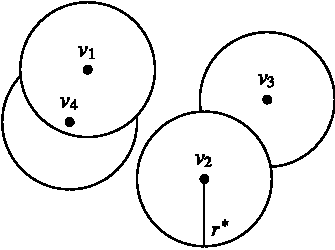
\includegraphics{./img/rand-clustering.pdf}
\caption{Clustering in Theorem \ref{theorem:clustering:1}}
\label{fig:3}
\end{figure}

The proof of Theorem \ref{theorem:clustering:1} is as follows:

\begin{description}
	\item[Bounded diameter] Consider two points $u$ and $v$. Since $r^*$ is fixed to be between $0$ and $\Delta / 2$, then if the two points belong in the same cluster, they must be not more than $r^*$ distance away from some point (which is the center of the ball). Therefore, by the triangle inequality they are not separated by more than $\Delta$. Therefore, the diameter of each cluster is at most $\Delta$.
	\item[Probability of cutting] Consider any two points $u$ and $v$. A vertex $w$ is said to settle $(u,v)$ if it is the \textbf{first} vertex in the order specified by $\sigma$ such that at least one of $u$ and $v$ belong to the $r^*$-ball centered at $w$. For every pair $(u,v)$, $w = u$ or $v$ is a settling vertex so at least one settling vertex must exist.
	Let $L_{uv}$ be the set of vertices $w$ such that at least one of $u$ and $v$ lie in the $r^*$-ball centered at $w$. Let $\pi$ denote vertices ordered as per the minimum of their distances to $u$ and $v$. Then, for some $k$, the set $L_{uv}$ will include the first $k$ vertices of $\pi$ and not include the remaining vertices. For a particular $w$, the probability that it settles $(u,v)$ is equal to the probability that $w \in L_{uv}$ and $w$ is first among the vertices of $L_{uv}$. If $w$ is in $L_{uv}$, then all vertices before $w$ in $\pi$ must belong to $L_{uv}$. Therefore, the probability that $w_i$, the $i^{th}$ vertex in $\pi$ settles $(u,v)$ satisfies, for fixed radius $r^*$,
	\begin{equation*}
		P (w_i \text{ settles } (u,v) | r^*) = \frac{1}{L_{uv}} \le \frac{1}{i}
	\end{equation*}
	Therefore, the probability that $u$ and $v$ are separated into different clusters (cut) is equal to:
	\begin{align}
		P (u,v \text{ lie in different clusters}) &= \mathbb{E}_{r^*} \left[\sum_{w_i \in \pi} P (w \text{ cuts } (u,v) | r^*) \right] \\
		&= \mathbb{E}_{r^*} \left[\sum_{w_i \in \pi} P (w_i \text{ settles } (u,v) | r^*) \cdot P (w_i \text{ cuts } (u,v) | r^*, w_i \text{ settles } (u,v)) \right] \\
		&\overset{(i)}{\le} \sum_i \frac{1}{i} P( d(w_i,u) \le r^* \le d(w_i,v) ) \label{ineq:1}\\
		&= \sum_i \frac{1}{i} \frac{d(w_i,v) - P( d(w_i,u)}{0.5 \Delta} \\
		&\le \sum_i \frac{1}{i} \frac{d(u,v)}{0.5 \Delta} \\
		&= H_n  \frac{d(u,v)}{0.5 \Delta} \\
		&\le 2 \log{n} \frac{d(u,v)}{\Delta}
	\end{align}
\end{description}
\end{proof}

\begin{theorem} \label{theorem:clustering:2}
Let $(X,d)$ be a metric space on n points, and $\Delta>0$. There is a probabilistic distribution of partitions $P$ of $X$ that satisfies the following properties:
\begin{enumerate}
    \item Each cluster $C$ in $P$ has diameter at most $\Delta$.
    \item For every $x\in X$ and $\rho>0$
    \begin{align*}
        Pr(B_\rho(x)\nsubseteq P(x)) \leq \alpha(x)\frac{\rho}{\Delta}
    \end{align*}
    where $\alpha(x)=O ( \log (\frac{|B_{\Delta}(x)|}{|B_{\Delta/8}(x)|}) ) $
\end{enumerate}

%The above clustering can be modified such that the probability that for every vertex $v$, the probability that it is cut by a ball of radius $\epsilon$ is proportional to $\epsilon$. In other words, smaller balls are more likely to lie entirely within a cluster than larger balls.
\end{theorem}
\begin{proof} {\color{red} [verify]}
The clustering is as follows:
\begin{enumerate}
\item Fix an $r \in [\Delta/4,\Delta/2]$ uniformly chosen from this set.
\item Pick a random permutation of points in $X$, called $\sigma$.
\item Iterate over points in $\sigma$ and for the $i^{th}$ point, form a ball of radius $r$ around this and allocate the points that have not yet been allocated to any point to this cluster. Iterate until no unclustered point remains.
\end{enumerate}

We'll consider $\rho<\Delta/8$ otherwise the guarantees are trivial. Consider a point $x$. Sort vertices of $X$ w.r.t distance from $x$. Call the sequence $\pi=\{u_1,u_2,\dots,u_n\}$. Define $A_i=d(u_i,x)+\rho$ and $B_i=d(u_i,x)-\rho$. Clearly $A_1<A_2<A_3,\dots,A_n$ and $B_1<B_2<B_3,\dots,B_n$.\\
Now consider if $x\in B_r(u_i)$ but $B_{\rho}(x)\nsubseteq B_r(u_i)$, then
\begin{align*}
    r &\in [A_i + \rho,B_i) \\
    \Rightarrow r &\in [A_i,B_i)
\end{align*}
Let the event $\beta_i$ denote the event that $u_i$ is the first vertex such that $r\geq A_i$. If $\beta_i$ and $r\geq B_i$, then:
\begin{enumerate}
    \item $B_\rho(x)\cap B_r(u_j)=\phi$ for $\forall j<i$
    \item $B_\rho(x)\subseteq B_r(u_i)$
\end{enumerate}
Thus
\begin{align*}
    Pr(B_{\rho}(x)\nsubseteq P(x)) \leq \sum_{1\leq i\leq n}Pr(\beta_i \; and \; A_i\leq r < B_i)
\end{align*}

Note that $Pr(\beta_i|r)<\frac{1}{i}$ and $Pr(A_i\leq r < B_i) \leq \frac{B_i-A_i}{\Delta/4}=8\rho/\Delta$. Now if $\Delta/2<A_i$ then $r<A_i$ (because $r\in[\Delta/4,\Delta/2]$), and so $\beta_i$ won't happen. Also, if $i>|B_\Delta(X)|$ then $u_i\notin B_{\Delta}(x)$ (since all vertices $u_i$ are sorted according to their distance to $x$) and hence
\begin{align*}
    A_i=d(u_i,x)-\rho \geq \Delta-\rho > \Delta/2 
\end{align*}
We use the fact that $\rho<\Delta/2$. And hence $Pr(\beta_i)=0$. Additionally, if $\Delta/4>B_i$ then $r>B_i$ and $Pr(A_i \leq r < B_i)=0$. Therefore if $i\leq |B_{\Delta/8}|$ then $u_i\in B_{\Delta/8}(x)$ and $B_i=d(u_i,x)+\rho \leq \Delta/8+ \rho < \Delta/4$ and hence $Pr(A_i\leq r <B_i)=0$. We conclude that:
\begin{align*}
    Pr(B_\rho(x)\nsubseteq P(x)) \leq \sum_{i=|B_{\Delta/8}(x)|}^{|B_{\Delta}|}\frac{1}{i}\cdot \frac{8\rho}{\Delta} = O\left(\log\frac{|B_{\Delta}|}{|B_{\Delta/8}(x)|} \cdot \frac{8\rho}{ \Delta } \right)
\end{align*}

%I read the proof of this theorem and writing it down here
%The clustering can be changed to pick $r^*$ from $[\Delta/4, \Delta/2]$ instead of just $[0, \Delta]$.
\end{proof}

This will be used to give a rounding algorithm for Problem~\ref{IP:CC3}.

\begin{proposition}[A $\log^2 (n)$ approximation to \ref{IP:CC3}]
The algorithm is as follows:
\begin{enumerate}
    \item Solve the LP relaxation of \ref{IP:CC3} optimally and denote its solution $\{ x_{uv}^* : (u,v) \in \binom{[n]}{2} \} \cup \{ Y_u^* : u \in [n] \}$. Define $\hat{x}_{uv} = x_{uv}^* + n^{-2}$.
    \item Randomly cluster the points as per Theorem~\ref{theorem:clustering:2} (with distance between points given by $\hat{x}_{uv}$) and consider $V^-$, all vertices connected by negative edges that are placed in the same cluster.
    \item Consider the subgraph formed by $V^-$ and the corresponding unsatisfied negative edges.
    \item Find a $2$-approximate vertex cover on this subgraph. For every negative edge, at least one of its end points will be removed and the resultant vertices will have all negative edge constraints satisfied.
    \item Consider the remaining vertices in the graph. Among these vertices, unsatisfied constraints are only because of points separated by a positive edge being put into different clusters. Let these vertices be denoted $V^+$.
    \item Once again find a $2$-approximate vertex cover on the subgraph formed by $V^+$ and the corresponding unsatisfied positive edges. Remove these vertices from the graph.
    \item Return the remaining vertices in the graph. There exists a clustering of these vertices with $0$ cost.
\end{enumerate}
\end{proposition}
\begin{proof}
{\color{red} change the negative edge analysis to reflect the modification in the algorithm}
\begin{enumerate}
	\item The first step of the algorithm is to solve the LP optimally. Consider its solution $\{ x_{uv}^* : (u,v) \in \binom{[n]}{2} \} \cup \{ Y_u^* : u \in [n]\}$. Recall that $\hat{x}_{uv}$ is defined as $x_{uv}^* + n^{-2}$.
	\begin{observation} The set of distances $\{ \hat{x}_{uv} \}$ forms a metric. This is because all distances are incremented by the same quantity.
	\end{observation}
	\item Since the set $\{ \hat{x}_{uv} \}$ forms a metric, one may find a randomized clustering $C$ (over all vertices) according to Theorem~\ref{theorem:clustering:2} in such a way that the diameter of each cluster is $\le \Delta$ which is chosen as $0.25$. Let the clustering be denoted $c_{uv}$ ($=0$ if $u$ and $v$ are in the same cluster and $1$ otherwise). The property of the clustering solution is that if $\hat{x}_{uv}$ is high, then the points $u,v$ are likely to lie in different clusters while if they are in the same cluster, they cannot be too far apart. This will be useful in rounding the optimal solution.

	\item Consider the vertices $V^-$ which are connected to at least one unsatisfied negative edge constraint and consider the subgraph $G^-$ formed by $V^-$ and these unsatisfied negative edges. For every vertex $v \in V^-$, there exists at least one other vertex in $u \in V^-$ with a negative edge to $u$, having $c_{uv} = 0$. Therefore, for such edges, the constraint that must necessarily be satisfied is
	\begin{equation*}
        Y_u^* + Y_v^* \ge 1 - x^*_{uv}
	\end{equation*}
	By the clustering in Theorem~\ref{theorem:clustering:2}, two points in the same cluster are not separated by a distance of more than $\Delta = 0.25$. Therefore, $c_{uv} = 0 \Rightarrow \hat{x}_{uv} \le 0.25 \Rightarrow x_{uv}^* \le 0.25 - \frac{1}{n^2}$. Therefore, we must necessarily have:
	\begin{equation} \label{eq:001}
		Y_u^* + Y_v^* \ge 0.75 + \frac{1}{n^2} \ge 0.75
	\end{equation}
	In Step 3 of the algorithm, we compute a $2$-approximate vertex cover over $G^-$. We consider a standard algorithm for vertex cover which is $2$-approximate.
	\begin{algorithm}[$2$-approximation for Vertex Cover] Pick an arbitrary negative edge constraint in this subgraph and discard both its end points. Choose any negative edge constraint that still remains unsatisfied and pick its end points. Repeat until no unsatisfied negative edge constraints remain.
	\end{algorithm}
	For each edge in $G^-$, define a random variable $a_e$ which is equal to $1$ if edge $e$ is chosen by the vertex cover algorithm and $0$ otherwise. Let $\OPT_-$ denote the component of the optimal solution corresponding to vertices in $V^-$. By the optimality of $Y^*_u$ we have,
	\begin{align}
	\OPT_- \ge \sum_{u \in V^-} Y^*_u &\ge \sum_{e = (u,v) \in G^-} (Y_{u}^* + Y_{v}^*) \cdot a_{e} \cdot c_{uv}, \nonumber\\
	&\overset{(i)}{\ge} \sum_{e = (u,v) \in G^-} 0.75 \cdot a_{e} \cdot c_{uv}. \label{eq:005}
	\end{align}
	where $(i)$ follows from Eq.~\eqref{eq:001}. On the other hand, the number of vertices removed by the algorithm in Step 4 is equal to twice the number of edges chosen in the vertex cover algorithm,
	\begin{equation*}
	\ALG_- = \sum_{e = (u,v) \in E^-} 2 \cdot a_{e} \cdot c_{uv} \le \frac83 \OPT_-.
	\end{equation*}
	where the last inequality follows from Eq.~\eqref{eq:005}. Therefore, among the set of vertices considered in Step 3 of the algorithm, the number of vertices discarded (in Step 4) is bounded by a constant fraction of the number of vertices discarded in the optimal solution.

% 	\item On the other hand, for positive edges, the situation is more precarious, but we will show that the same clustering (which is done for the entire metric) can be used to round effectively.
% 	For any positive edge, $(u,v) \in E^+$, $u$ and $v$ must belong in the same cluster for the cost of the clustering to be equal to $0$. They must also satisfy the constraint:
% 	\begin{equation} \label{eq:002}
% 		Y_u^* + Y_v^* \ge x_{uv}^*
% 	\end{equation}
% 	Observe that for two points separated by a distance $x_{uv}^*$, the clustering from Theorem~\ref{theorem:clustering:1} separates them into different clusters with probability $\le (8 \log{n}) x_{uv}^*$. In other words, $P(c_{uv} = 1 | x_{uv}^*) \le (8 \log n) x_{uv}^*$. %{\color{red} Let us apply the vertex cover algorithm as in the previous section for positive edges that have $c_{uv} = 1$}.
% 	For a particular run of the vertex cover algorithm, OPT and SOL satisfy:
% 	\begin{align*}
% 		OPT &\ge \sum_{u \in V^+} Y^*_u \ge \sum_{e_i = (u_i,v_i) \in E^+ } (Y_{u_i}^* + Y_{v_i}^*) \cdot a_{i} \cdot c_{u_iv_i} \\
% 		SOL &= \sum_{e_i = (u_i,v_i)} (d_{u_i} + d_{v_i}) \cdot a_{i} \cdot c_{u_iv_i}
% 	\end{align*}
% 	We want to show that OPT is not too small compared to SOL, or in other words, we want to use the fact that for some $e_i$ if $Y_{u_i}^*$ and $Y_{v_i}^*$ are both small, then $x_{uv}^*$ must be small (Eq.~\eqref{eq:002}). Therefore, the two points will be likely to have $c_{uv} \gets 0$ and therefore, both $d_{u_i}$ and $d_{v_i}$ will be made $0$ WHP. Then,
% 	\begin{proposition} \label{prop:1}
% 	\begin{equation}\label{eq:003}
% 		R \triangleq \mathbb{E} \left[ \frac{\sum_{e_i = (u_i,v_i) \in E^+} (d_{u_i} + d_{v_i}) \cdot a_{i} \cdot c_{u_iv_i}}{\sum_{e_i = (u_i,v_i) \in E^+} (Y_{u_i}^* + Y_{v_i}^*) \cdot a_{i} \cdot c_{u_iv_i}} \right] \le \mathbb{E} \left[ \max_{i} \left( \frac{(d_{u_{i}} + d_{v_{i}}) \cdot a_{i} \cdot c_{u_iv_i} }{(Y_{u_i}^* + Y_{v_i}^*) \cdot a_{i} \cdot c_{u_iv_i}}\right) \right]
% 	\end{equation}
% 	\end{proposition}
% 	\begin{proof}
% 	\textbf{Inductive Hypothesis}: Let $A_1,A_2,\cdots,A_n$ and $B_1,B_2,\cdots,B_n$ be positive. Then 
% 	\begin{equation}\label{eq:004}
% 	    \frac{A_1+A_2+...+A_n}{B_1+B_2+...+B_n} \leq \max_i \left(\frac{A_i}{B_i} \right)
% 	\end{equation}
% 	\textbf{Base Step}: Eq.~\eqref{eq:004} is trivially true for $n=1$.\\
% 	\textbf{Inductive Step}: Let the equation be true for some $n=k$. Let the $r = \argmax_i A_i/B_i$.
% 	We prove the equation is also true for $n=k+1$. Assume $\sum_{i\leq k} A_i = A'$, and $\sum_{i\leq k} B_i = B'$. There are two cases:
% 	\begin{description}
% 	    \item[Case I: $\frac{A_{k+1}}{B_{k+1}} \ge \frac{A'}{B'}$]. We prove by contradiction that $\frac{A_{k+1}+A'}{B_{k+1}+B'} \leq \frac{A_{k+1}}{B_{k+1}}$. Suppose this is false. Then,
% 	    \begin{align*}
%             \frac{A_{k+1}+A'}{B_{k+1}+B'} &> \frac{A_{k+1}}{B_{k+1}}\\
% 	        \Rightarrow\ (A_{k+1}+A') \cdot B_{k+1} &> (B_{k+1}+B') \cdot A_{k+1}\\
% 	        \Rightarrow\ A_{k+1} \cdot B_{k+1} + A' \cdot B_{k+1} &> A_{k+1} \cdot B_{k+1} + B' A_{k+1}\\
% 	        \Rightarrow\ \frac{A'}{B'} &>  \frac{A_{k+1}}{B_{k+1}}
% 	    \end{align*}
% 	    Thus, a contradiction.
% 	    \item[Case II: $\frac{A_{k+1}}{B_{k+1}} < \frac{A'}{B'}$] A similar argument results in $\frac{A_{k+1}+A'}{B_{k+1}+B'} \leq \frac{A'}{B'} \leq \frac{A_{r}}{B_{r}}$
% 	\end{description}
%  	\end{proof}
	 
%     Observe that with probability at most $(8 \log{n}) x_{uv}^*$, $c_{uv}$ is 1 ($u$ and $v$ lie in different clusters). Thus, $d_u$ and $d_v$ are $1$ with probability not exceeding this quantity (since they are surely $0$ if $c_{uv} = 0$). Using this, Eq.~\eqref{eq:002}, we get:
% 	\begin{equation*}
% 		R \le \mathbb{E} \left[ \frac{d_{u_i} + d_{v_i}}{x^*_{uv}} \right] \le 2 \cdot (8 \log n)
% 	\end{equation*}
	
	\item We now move on to the analysis for positive edge constraints. Recall that $\hat{x}_{uv}$ is defined as $x_{uv}^* + n^{-2}$. 
	%The difference now is that our cost function has value: $\sum_{u} (Y_{u}^* + \frac{1}{n^2})$, where $Y_{u}^*$ is the value in the optimal solution.\\
	%The main problem we are trying to solve is when a positive edge indeed gets cut by our clustering algorithm.
	\begin{observation} The solution $\{ \hat{x}_{uv} \} \cup \{ Y_u^* + n^{-2} \}$ forms a feasible solution to the LP relaxation of \ref{IP:CC3}. The set $\hat{x}_{uv}$ forms a metric and $Y_u^* + Y_v^* + 2n^{-2} \ge \hat{x}_{uv} + n^{-2} \ge \hat{x}_{uv}$.
	\end{observation}
	Let us first define $\hat{Y}_u$ as follows
	\begin{align*}
	    \hat{Y}_{u}=\frac{Y_u^* + n^{-2}}{\frac{1}{2^r}},
	\end{align*}
	where $\frac{1}{2^{r}} < \underset{v : c_{uv} = 1}{\min} \hat{x} (u,v) \le \frac{1}{2^{r-1}}$. In Step 5 of the algorithm, the remaining vertices are denoted $V^+$. For $u \in V^+$, there exists at least one other vertex $v \in V^+$ that has not been removed in Step 4 of the algorithm, such that $(u,v)$ is a positive edge and $c_{uv} = 1$. Consider $G^+$, the subgraph formed by vertices in $V^+$ and the unsatisfied positive edges between these vertices. For every edge $(u,v)$ in $G^+$, $\hat{Y}_u$ will satisfy the constraint
	\begin{align} \label{eq:vcconstraint}
	    \hat{Y}_{u} + \hat{Y}_{v} &\geq 1.
	\end{align}
	For any vertex $u \in V^+$, such that $\exists v : c_{uv} = 1$, the expected value $\mathbb{E} [ \hat{Y}_{u} ]$ is,
	\begin{align}
	    \mathbb{E} [\hat{Y}_{u}] &= \sum_{r \in [2 \log(n)]} 2^{r} \cdot (Y_u^* + n^{-2}) \cdot \mathrm{Prob} \left( 2^{-r} < \min_{v : c_{uv} = 1} \hat{x}_{uv} \le 2 \cdot 2^{-r} \right) \nonumber\\
	    % that is not correct right? If a radius r is cut, all larger radii are cut. Not all smaller radii. Sure.
	    % yes you are right. But there exists a vertex at a distance less than 1/2^{r-1} which is cut right? If that guy is cut, all higher radii are cut. Ok.
	    &\le \sum_{r \in [2 \log(n)]} 2^{r} \cdot (Y_u^* + n^{-2}) \cdot \mathrm{Prob} \left( \min_{v : c_{uv} = 1} \hat{x}_{uv} \le 2 \cdot 2^{-r} \right) \nonumber\\
	    &\le \sum_{r \in [2 \log(n)]} 2^{r} \cdot (Y_u^* + n^{-2}) \cdot \mathrm{Prob} \left( \text{ball of radius } 2 \cdot 2^{-r} \text{ is cut} \right) \nonumber \\
	    &= \sum_{r \in [2 \log(n)]} 2^r \cdot (Y_u^* + n^{-2}) \cdot \frac{2}{2^r} \cdot \frac{2 \log{n}}{\Delta} \nonumber \\
	    &= 4 \log^2(n) \left( \frac{1}{n^2}+Y_u^* \right) \label{eq:apx1}
	\end{align}
	Recall the definition of $\hat{Y}_u$ as $2^r (Y_u^* + n^{-2} )$ where $2^{-r} < \underset{v : c_{uv} = 1}{\min} x_{uv^*} \le 2 \cdot 2^{-r}$. The $\hat{Y}_u$'s satisfy Eq.~\eqref{eq:vcconstraint}.
	
	We claim that we can find $Z_u \in \{ 0,1 \}$ such that Eq.~\eqref{eq:vcconstraint} is satisfied and \begin{equation*}
	    \mathbb{E} \left[ \sum_{u \in V^+} Z_u \right] \le 2 \cdot \mathbb{E} \left[ \sum_{u \in V^+} \hat{Y}_u \right]
	\end{equation*}
	This is because there exists an algorithm which is $2$-approximate with respect to the fractional optimal solution of the vertex cover constraints satisfied by $\hat{Y}_u$. Even if such an algorithm does not exist, the factor is at most $4$ because one can use any vertex cover algorithm that is $2$-approximate and generate a solution that is not more than twice the optimal integral solution which itself is not more than twice the optimal fractional solution (since the integrality gap of vertex cover is $\le 2$).

	Therefore, the overall cost of our solution is,
	\begin{align*}
	    \ALG_+ = \mathbb{E} \left[ \sum_{u \in V^+} Z_u \right] &\le 2 \cdot \mathbb{E} \left[ \sum_{u \in V^+} \hat{Y}_{u} \right]\\
	    &\overset{(i)}{\le} 2 \cdot 4 \log^2 (n) \sum_{u \in V^+} \left( \frac{1}{n^2}+Y_u^* \right)\\
	    &\leq 8 \frac{\log^2(n)}{n}+ 8 \log^2(n) \cdot \left( \sum_u Y_u^* \right)\\
	    &\le 8 \frac{\log^2(n)}{n} + 8 \log^2(n) \cdot \OPT_+
	\end{align*}
	where in the last inequality, $\OPT_+$ is the cost accumulated by the component of the optimal solution corresponding to vertices in $V^+$ and $(i)$ follows from Eq.~\eqref{eq:apx1}.
	%We now show that the term $\frac{8 \log^2 (n)}{n}$ doesn't make the approximation ratio unbounded when the optimal solution has $0$ cost. When the OPT is 0, this means that the solution of the fractional optimal solution the IP is also $0$. Therefore, clustering algorithm also makes SOL=0. When the OPT is not 0, the rounded optimal solution will be at least 1 (i.e., at least one vertex will be chosen as rounded optimal as it's $\geq$ OPT, and given OPT is not 0). In this case, $O(8 \frac{\log^2(n)}{n}) = o(1)$ \\
	
	%Replacing $\frac{1}{n^2}$ by $\frac{1}{n^{\epsilon}}, \epsilon>0$, we'll get:
	%\begin{align*}
	%    SOL &\leq (\epsilon)*4\frac{log^{2}(n)}{n^{\epsilon-1}}+ (\epsilon)*4log^{2}(n)OPT
	%\end{align*}
\end{enumerate}
\end{proof}

\section{Bi-criterion problem}
The \ref{IP:CC4} can't be approximated to $(\alpha, \beta)$ for any $1\leq \alpha<2$. Consider the same construction as in Section 2. The objective here is to select m points such that removing of $m$ points give the most optimal clustering cost possible. If we choose $m$= $|$vertex cover$|$ of the graph $G'$, then having a $(\alpha, \beta)$, where $\alpha<2$ would mean solving the vertex cover with better than 2 approximation ratio, which isn't possible. Hence, $\alpha \geq 2$.\\

Now consider the following LP:
%Consider \ref{IP:CC4}. Let's say we solve the IP optimally. Consider the constraints involving only the bad edges, i.e., $x_{uv\in E^+}=1$ and $x_{uv\in E^-}=0$, we'll get the following LP:
\begin{alignat}{3} \label{IP:CC5}
		&\text{Find: } && \min \sum_{(u,v) \in E} z_{uv}, \nonumber\\
		&\text{Subject to:} \quad && \forall u,v \in V,\ Y_u + Y_v + z_{uv} \ge 1, \nonumber\\
		& && \sum_{u} Y_u \le m \nonumber \\
		& && \forall u,v \in [n],\ z_{uv} \in \{ 0,1 \},\nonumber\\
		& && \forall u \in [n],\ Y_u \in \{ 0,1 \}. \tag{IP4}
\end{alignat}

\begin{algorithm}[$(3,3)$ bi-criteria approximation for \ref{IP:CC5}] \label{alg:IP:CC5} An $(a,b)$-bicriteria approximation means that the budget of number of vertices removed is violated by a factor of $a$ and the resultant solution we get is within a factor of $b$ of the optimal solution to the problem. A $(3,3)$ bi-criteria approximation to \ref{IP:CC5} is as follows:
\begin{enumerate}
    \item Find the optimal solution of the LP-relaxation of \ref{IP:CC5}. Denote it as $\{ z_{uv}^* \} \cup \{ Y_u^* \}$.
    \item Round each $Y_u^* > 1/3$ to $1$ and each $Y_u^* \le 1/3$ to $0$.
    \item Set the unsatisfied $z_{uv}^*$'s to $1$.
\end{enumerate}
\end{algorithm}
\begin{proof}
It is apparent that the budget used by this algorithm by the rounded $Y_u$'s will not exceed $3m$. The cost accumulated by the algorithm is equal to $\sum_{(u,v) \in E} \mathbbm{1}_{Y_u^* \le 1/3 \text{ and } Y_v^* \le 1/3}$. The optimal cost is lower-bounded by the optimal fractional cost equal to
\begin{align*}
    \OPT \ge \sum_{(u,v) \in E} z_{uv}^* &\ge \sum_{(u,v) \in E} 1 - Y_u^* - Y_v^* \\
    &\ge \frac{1}{3} \sum_{(u,v) \in E} \mathbbm{1}_{Y_u^* \le 1/3 \text{ and } Y_v^* \le 1/3} = \frac{1}{3} \ALG
\end{align*}
If we round $Y_u^*$ at a threshold of $k^{-1}$ (in the above $k = 3$), we get a $\left(k,\frac{k}{k-2}\right)$ bi-criteria approximation for \ref{IP:CC5}.
\end{proof}

%What it means is that given the optimal solution to the IP, we can find a (3,3) approximation. In fact, replace 3 by $k$ and we'll have a $\left(k,\frac{k}{k-2}\right)$ approximation for \ref{IP:CC5}.\\

\begin{proposition}[A $(O(\log^2(n)),O(\log (n)))$ bi-criteria randomized approximation to \ref{IP:CC4}]
The algorithm is as follows:
\begin{enumerate}
    \item Solve the LP relaxation of \ref{IP:CC4} optimally and denote its solution $\{ x_{uv}^* : (u,v) \in \binom{[n]}{2} \} \cup \{ z_{uv}^* : (u,v) \in \binom{[n]}{2} \} \cup \{ Y_u^* : u \in [n] \}$. Define $\hat{x}_{uv} = x_{uv}^* + n^{-2}$ and $\hat{z}_{uv} = z_{uv}^* + n^{-2}$.
    \item Randomly cluster the points as per Theorem~\ref{theorem:clustering:2} (with distance between points given by $\hat{x}_{uv}$). Let $V^-$ denote vertices connected by negative edges that are placed in the same cluster. We define $G^-$ as the graph over $V^-$ spanned by the unsatisfied negative edges between these vertices.
    \item Algorithm \ref{alg:IP:CC5} gives a $(3,3)$ bi-criteria approximation for \ref{IP:CC5} which gives a collection of $3m$ vertices, which when removed is within a factor $3$ of the optimal number of remaining edges when the optimal $m$ vertices were removed. We use the same algorithm on graph $G^-$ with a budget of some $m_1 \le m$ and remove the vertices (and edges) it outputs from the graph. Due to the suboptimal clustering, we are able to make a weaker guarantee that the resultant clustering is $(4,4)$ bi-criteria approximate. This is indirectly due to the integrality gap of the optimization problem being solved.
    %For every negative edge, at least one of its end points will be removed or $z_{uv}^*$ be made 1 and the resultant vertices will have all negative edge constraints satisfied.
    \item Consider the remaining vertices in the graph. Among these vertices, unsatisfied constraints are only because of points separated by a positive edge being put into different clusters. Let these vertices be denoted $V^+$. Put together with their unsatisfied positive edges, let us denote this subgraph as $G^+$.
    \item We now use Algorithm \ref{alg:IP:CC5} again on this graph with $m = $ $(\mathcal{O}(\log(n)),\mathcal{O}(\log^2(n)))$ bi-criteria approximation on the subgraph formed by $V^+$ and the corresponding unsatisfied positive edges. Remove these vertices from the graph.
    \item Return the remaining vertices in the graph. There exists a clustering of these vertices with $(O(\log(n)),O(\log^2(n)))$ bi-criteria approximation.
\end{enumerate}
\end{proposition}
\begin{proof}
The proof follows very similar to the proof for Proposition 8.
\begin{enumerate}
    \item Let $\Delta=0.25$. Consider the vertices $V^-$ which are connected to at least one unsatisfied negative edge constraint and consider the subgraph $G^-$ formed by $V^-$ and these unsatisfied negative edges. For every vertex $v \in V^-$, there exists at least one other vertex in $u \in V^-$ with a negative edge to $u$, having $c_{uv} = 0$. Therefore, for such edges, the constraint that must necessarily be satisfied is
	\begin{equation*}
        Y_u^* + Y_v^* + z_{u}^* \ge 1 - x^*_{uv}
	\end{equation*}
	By the clustering in Theorem~\ref{theorem:clustering:2}, two points in the same cluster are not separated by a distance of more than $\Delta = 0.25$. Therefore, $c_{uv} = 0 \Rightarrow \hat{x}_{uv} \le 0.25 \Rightarrow x_{uv}^* \le 0.25 - \frac{1}{n^2}$. Therefore, we must necessarily have:
	\begin{equation} \label{eq:006}
		Y_u^* + Y_v^* + z_{u}^* \ge 0.75 + \frac{1}{n^2} \ge 0.75
	\end{equation}
	Also let $\hat{m}$ be used to denote the partial constraint:
	\begin{align*}
	    \sum_{u\in V^-} Y_u^* \leq \hat{m}
	\end{align*}
	In Step 3 of the algorithm, we compute a $(4,4)$ bi-criteria approximation over $G^-$. We apply Algorithm \ref{alg:IP:CC5} which is a $(4,4)$ bi-criteria approximation here.
	\begin{algorithm}[$(4,4)$ bi-criterion approximation] This directly follows from Algorithm \ref{alg:IP:CC5} and a bound on the integrality gap. For each negative edge constraint, round the variable $Y_u^*$ or $z_u^*$ to 1 if their value is $\geq 1/4$. Else round them to $0$.
	\end{algorithm}
	%For each edge in $G^-$, define a random variable $a_e$ which is equal to $1$ if edge $e$ is chosen by the vertex cover algorithm and $0$ otherwise.
	Let $\OPT_-$ denote the component of the optimal solution corresponding to edges in $G^-$. By the optimality of $z^*_u$ we have,
	\begin{align}
	\OPT_- \ge \sum_{u,v \in V^-} z^*_{uv} \label{eq:007}
	\end{align}
	The cost of our rounded solution by the algorithm in Step 4 is:
	\begin{equation*}
	\ALG_- \leq 4 \left( \sum_{u,v \in V^-} z^*_{uv} \right) \leq 4(\OPT_-)
	%\ALG_- = \sum_{e = (u,v) \in E^-} 2 \cdot a_{e} \cdot c_{uv} \le \frac83 \OPT_-.
	\end{equation*}
	where the last inequality follows from Eq.~\eqref{eq:007}.
	Also, we end up approximating $\sum_{u\in V^-}Y_u^*$. Let the rounded value of $Y_u^*$ be $Y_u^r$. We get:
	\begin{align*}
	    \sum_{u\in V^-} Y_u^r \leq 4(\sum_{u\in V^-} Y_u^*) \leq 4\hat{m}
	\end{align*}
	Therefore, among the set of vertices considered in Step 3 of the algorithm, the number of vertices discarded (in Step 4) is bounded by a constant factor of the number of vertices allowed to be discarded in the optimal solution, and therefore we get a (4,4) bi-criteria approximation.
	\item We now move on to the analysis for positive edge constraints. Recall that $\hat{x}_{uv}$ is defined as $x_{uv}^* + n^{-2}$.\\
	Let us first define $\hat{Y}_u$ as follows
	\begin{align*}
	    \hat{Y}_{u}=\frac{Y_u^* + n^{-2}}{\frac{1}{2^r}},\\
	\end{align*}
	where $\frac{1}{2^{r}} < \underset{v : c_{uv} = 1}{\min} \hat{x} (u,v) \le \frac{1}{2^{r-1}}$.
	We define $\hat{z}_{uv}$ as follows:
	\begin{equation*}
	    \hat{z}_{uv} = 
	    \begin{cases}
	    \frac{z_{uv}^*}{x^*_{uv}}, \quad &c_{uv}=1,\\
	    0 &\text{otherwise}.
	    \end{cases}
	\end{equation*}
    Hence, we have the inequality:
    \begin{equation*}
        \mathbb{E} [\hat{z}_{uv}] = \mathcal{O} \left(\frac{ \log (n)\cdot z^*_{uv}}{\Delta} \right).
    \end{equation*}
	In Step 5 of the algorithm, the remaining vertices are denoted $V^+$. For $u \in V^+$, there exists at least one other vertex $v \in V^+$ that has not been removed in Step 4 of the algorithm, such that $(u,v)$ is a positive edge and $c_{uv} = 1$. Consider $G^+$, the subgraph formed by vertices in $V^+$ and the unsatisfied positive edges between these vertices. For every edge $(u,v)$ in $G^+$, $\hat{Y}_u$ will satisfy the constraint
	\begin{align} \label{eq:IP3normalized}
	    \hat{Y}_{u} + \hat{Y}_{v} + \hat{z}_{uv} &\geq 1.
	\end{align}
	Our approach is identical to the proof of Proposition 6 proof. One can work out that,
	\begin{align*}
	    \mathbb{E} [\hat{Y}_{u}] &= 4 \log^2(n)\left(\frac{1}{n^2} + Y_u^* \right)\\
	    \mathbb{E} [\hat{z}_{uv}] &= O \left(\frac{ \log(n)\cdot z^*_{uv}}{\Delta} \right)
	\end{align*}
	We now claim that we can find a solution to Equation~\ref{eq:IP3normalized}, that is a $(3,3)$ bi-criteria approximation. We use Algorithm \ref{alg:IP:CC5} and round $\hat{Y}_u$ and $\hat{z}_{uv}$ to 1 if their value is $\geq$ 1/3, else to $0$. Comparing the expected cost of rounded solution calculated through our algorithm to the fractional optimal solution of the IP with constraint satisfied by $\hat{Y}_u$ and $\hat{z}_{uv}$, we get:
	\begin{align*}
	    \mathbb{E}[\ALG_+] \leq \mathbb{E} [\sum_{e=(u,v)\in V^+} 3(\hat{z}_{uv})] &= \mathcal{O} \left( \frac{ \log(n)}{\Delta} \right) \cdot \sum_{(u,v) \in E} z^*_{uv},\\
	    &\leq \mathcal{O} \left(\frac{\log(n)}{\Delta} \right) \cdot \OPT_+.
	    %3(4 \log^2(n) \cdot \sum_{e=(u,v)\in V^+} \left(\frac{1}{n^2} + z_{uv}^* \right))
	    %&\leq 12 \log^2(n) + 12 \log^2(n)\cdot OPT_+
	\end{align*}
	where in the last inequality, $\OPT_+$ is the cost accumulated by the component of the optimal solution corresponding to the misclassified edges in $G^+$ in the optimal solution.
	
	Let $Y_u^r$ be the rounded value of $Y_u^*$. And let $m_1$ be the $m$-budget used for vertices in $G^+$.
	\begin{align*}
	    \sum_{u\in V^+} Y_u^*\leq m_1
	\end{align*}
	Then we have:
	\begin{align*}
	    \mathbb{E} \left(\sum_{u\in V^+} Y_u^r \right) &\le \mathbb{E} \left( \sum_{u\in V^+} 4\hat{Y}_u \right)\\
	    &=4\cdot 4 \log^2(n) \cdot \sum_{u\in V^+}\left(\frac{1}{n^2} + Y_{u}^* \right)\\
	    &\leq 16\frac{\log^2(n)}{n} + 16 \log^2(n)\cdot m_1
	\end{align*}
	
	Hence we have a $(\mathcal{O}(\log(n)), \mathcal{O}(\log^2(n)))$ bi-criterion approximation to \ref{IP:CC5}.
\end{enumerate}

\end{proof}

% \section{Hardness of Problem 3 from multicut}

% Consider an instance of multicut with pairs of $\{ s_i,t_i \}$ terminal pairs on a graph $G = (V,E)$. The vertices of this graph are colored black in Fig.~\ref{fig:5}. The instance of Problem 3 constructs a graph with $|V| + |E|$ vertices with a vertex added that splits every edge in two (white vertices in Fig.~\ref{fig:5}). Every $s_i$-$t_i$ pair is discouraged from lying in the same cluster by adding $W$ parallel length $2$ paths between these vertices with one being $+$ and the other being $-$ (thick red edge in Fig.~\ref{fig:5}). The cost of any clustering is invariant to which side of the white vertex is the cut being made . Therefore, we may assume that the edges cutting the optimal clustering
% have white vertices all to one side and black vertices on the other side. Then the cost of Problem $3$ is to find the clustering with least edges cutting and the optimal choice of vertices to remove would be the white vertices that all lie on the same side of the clustering boundary. The number of vertices to remove is exactly equal to the number of edges in the optimal multicut of $G$.

% \begin{figure}[ht]
% \centering
% 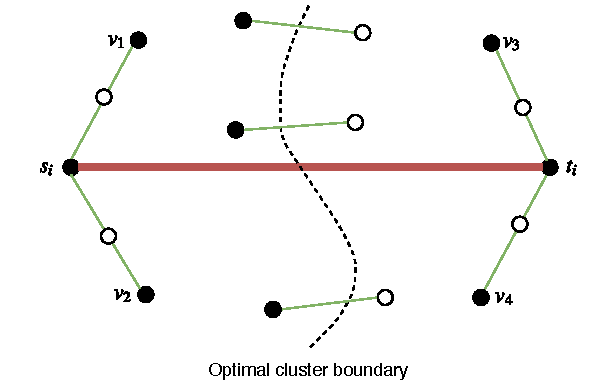
\includegraphics{./img/multicut-multipartite.pdf}
% \caption{Instance of Problem 3 with $|V| + |E|$ vertices}
% \label{fig:5}
% \end{figure}

\section{Problem 4 as hard as multicut}

We first show the hardness in terms of approximating the cost for any $m$ (refer $\ref{IP:CC4}$).
Consider an undirected simple graph instance $G$ of Multicut problem with $k$ source-sink pairs represented as $(s_i,t_i)$. Connect each $s_i,t_i$ with $v_1,v_2,\cdots, v_{n^3}$, such that the edge $s_i,v_j$ is marked $+1$, and the edge $t_i,v_j$ is marked $-1$. Now add $m$ more vertices, say $u_1,u_2,\cdots,u_m$, and connect each $u_i$ with each vertices in $G$ in the following way:\\
Let's consider the vertex $q\in V(G)$
\begin{enumerate}
    \item Make similar connections like $l_1,l_2,\cdots, l_{n^3}$ between $u_i$, and $q$ such that the edge $q,l_j$ is marked $+1$, and the edge $u_i,l_j$ is marked $-1$.
    \item Also make similar connections, say $p_1,p_2,\cdots,p_{n^3}$, and mark both the edges $q,p_j$ and $u_i,p_j$ as $+1$.
\end{enumerate}
\begin{proof}
Consider the vertex $q$ and $u_i$:
\begin{enumerate}
    \item If they are in same cluster, the cost is high due to vertices $l_k(s)$, irrespective where we cluster these $l_k(s)$.
    \item If we don't put $q$ and $u_i$ in same cluster, then cost is very high due to vertices $p_j(s)$.
\end{enumerate}
Hence, if asked to calculate the most optimal cost possible after removing any of $m$ vertices of this newly constructed graph, the best strategy would be to remove the vertices $u_1,u_2,\cdots,u_m$ as they add very highly to the cost irrespective of where we place them. And after removing these, the optimal cost of the graph is same as the multicut optimal cost of graph $G$.
\end{proof}

Now we show hardness in terms of approximating $\sum_uY_u^*$ (refer \ref{IP:CC4})\\
\begin{proposition}
Consider an undirected simple graph $G=(V,E)$. Also let there be $k$ pairs of $s_i\in V,t_i\in V$ source-sink pairs. Define the problem $Vertex-MultiCut$ as of finding minimum number of vertices so that each source-sink pair don't lie in the same connected component.\\
The problem $Vertex-MultiCut$ is as hard as $MultiCut$ problem.
\end{proposition}
\begin{proof}
Convert each vertex into a clique of large size, say $n^3$, where $n=|V|$.
\end{proof}